% vim: set spell:

\chapter{Assessment Pipeline}

\begin{quotation}

\footnotesize\sffamily\itshape

\begin{flushright}

/* War is peace. Verbosity is silence. MS\_VERBOSE is deprecated. */

\smallbreak

\upshape

--- DAVID HOWELLS, Linux Source Code (2012)

\end{flushright}

\end{quotation}

When a student makes a submission, it needs to be assessed. The process of
assessment is specified by the teaching staff, and may consist of a series of
steps --- an assessment pipeline.

Each step of the pipeline is a computer program exposing a particular
interface. The combination of these programs forms a pipeline, taking the
student submission in at one end, and producing ``student-friendly'' feedback
at the other.

A student submission consists of a series of files. Some of these files may be
expected to specify computer programs. Let a static assessment be an assessment
where we analyse the submitted files, without executing what we expect to be
student programs. Let a dynamic assessment be an assessment where we attempt to
execute these programs.

The primary form of assessment is static assessment. A static assessment will
often facilitate a subsequent dynamic assessment. For instance, by ensuring
that the student has submitted all relevant files, or by compiling student
programs.  Although the distinction between static and dynamic assessment is
sometimes rather subtle, we provide this abstraction, and leave it to the user
to judge what belongs where, according to the problem at hand.

The direct output of a static or dynamic assessment may bee to obscure or too
detailed for a student to benefit from it (see also
\referToSection{assessment-in-computer-science:feedback}). We introduce a
feedback refinement process, intended for transforming this ``raw'' feedback
into ``student-friendly'' feedback. This refinement process may further be
parametrized by the current student and course progress.

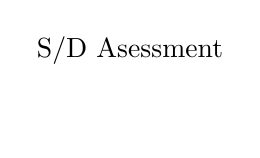
\begin{tikzpicture}
\draw (0,0) {};
\draw (0,1) node {S/D Asessment};
\end{tikzpicture}
